108. Возможны два случая расположения данных углов: оба внутри образующегося при пересечении треугольника, или один угол внутри, а другой --- снаружи. В первом случае картинка имеет следующий вид:
\begin{figure}[ht!]
\center{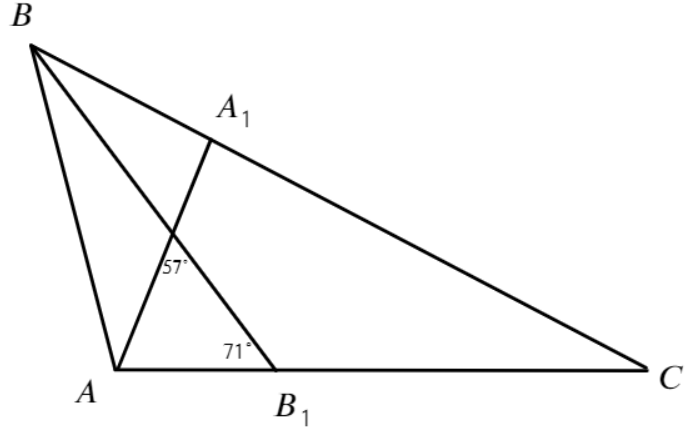
\includegraphics[scale=0.35]{g108.png}}
\end{figure}\\
Найдём $\angle A_1AC=180^\circ-57^\circ-71^\circ=52^\circ,$ значит $\angle A=2\cdot52^\circ=104^\circ.$ Тогда $\angle ABB_1=180^\circ-104^\circ-71^\circ=5^\circ,\ \angle B=2\cdot5^\circ=10^\circ,\ \angle C=180^\circ-104^\circ-10^\circ=66^\circ.$\\
Во втором случае картинка имеет следующий вид:\\
\begin{figure}[ht!]
\center{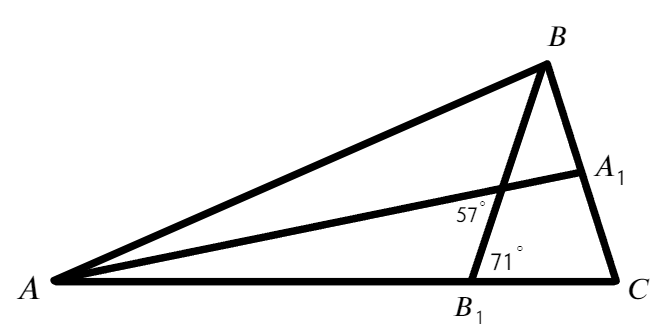
\includegraphics[scale=0.35]{g1082.png}}
\end{figure}\\
Найдём $\angle A_1AC=180^\circ-57^\circ-(180^\circ-71^\circ)=14^\circ,$ значит $\angle A=2\cdot14^\circ=28^\circ.$ Тогда $\angle ABB_1=180^\circ-28^\circ-109^\circ=43^\circ,\ \angle B=2\cdot43^\circ=86^\circ,\ \angle C=180^\circ-28^\circ-86^\circ=66^\circ.$\\
